\chapter{APPENDIX 1: Gaussian Integration}


The Gaussian integration method as applied in the model, is based on a study by Goudriaan
(1986). In the following text this method will be briefly explained.

The rate of crop photosynthesis can be computed from the photosynthesis - light response
curve of individual leaves, the incoming radiation and the leaf area index. Leaf area
distribution, extinction and reflection coefficients must also be known since they influence
the distribution of the available radiation. This computational problem was essentially solved
by De Wit (1965). He applied a stratification of the leaf canopy, calculated the absorbed
radiation and the corresponding rates of photosynthesis of sunlit and shaded leaves in each
layer. The contributions of the individual layers  were added to find the rate of crop
photosynthesis. This procedure was repeated every 15 minutes to obtain the daily total of
crop photosynthesis. This procedure is lucid and flexible, but rather time consuming.
Therefore, its use during an entire season as one would want in simulation of crop growth,
might become problematic.

For application in such models Goudriaan and Van Laar (1978) developed a summary model
for the daily total of crop photosynthesis, based on a semi-empirical equation, fitted to
computer output of the detailed model.

Usually integration in time or in spatial dimension is done by means of the well-known
numerical methods such as Eulerian (rectangular), Simpson or Runga - Kuta methods. These
methods are excellent and generally applicable because they permit feedback of the
integrated value (state variable) on the rate itself. But when there is no such feedback, and
the profile of the rate is known on forehand, a method, devised by the German
mathematician Gauss, is much more efficient and accurate. 

Several examples of processes where this feedback is absent can be defined in the crop
growth modeling. In those cases the Gaussian integration can be applied. Examples in the
WOFOST model where this method is used:
\begin{itemize}
\item the calculation of crop photosynthesis from a known light profile. Integration
    of the light response curve over the leaf area depth of the canopy. 
\item integrate an independently given diurnal course (for example assimilation) into
    a daily total.
\end{itemize}

Gaussian integration is explained in several textbooks on numerical methods (Lanczos, 1957;
Scheid, 1968). The basic idea is to compute the rate at positions in the total integration
interval area as representative as possible. In its simplest form, the Gaussian one-point
method, one single value of the rate is taken halfway through the integration interval. It
gives a more accurate result than the rectangular integration method, because errors left and
right of the evaluation point in the center practically cancel.

In a more formal analysis the integration interval is normalized to unity, and centralized
between x=-$\frac{1}{2}$ and x=$\frac{1}{2}$. The polynomial given by 
y=a+bx+cx$^{{\rm 2}}$+dx$^{{\rm 3}}$ ... will have value
a at the center point x=0. Therefore, the integrated value obtained by the one point
Gaussian integration, will also be equal to a. Analytical integration of the polynomial term
by term shows that the integrals of all odd terms disappear around x=0, That means that
the one-point method not only exactly integrates $y=a$, but also $y=a+bx$. Similarly the two-point 
method will exactly $integrate y=a+bx+cx^{{\rm 2}}$ and $y=a+bx+cx^{{\rm 2}}$+dx$^{{\rm 3}}$. 
The next step is the three point method which will enable exact integration of the fourth order 
term (and automatically the fifth as well).
 
\begin{figure}
 \centering
  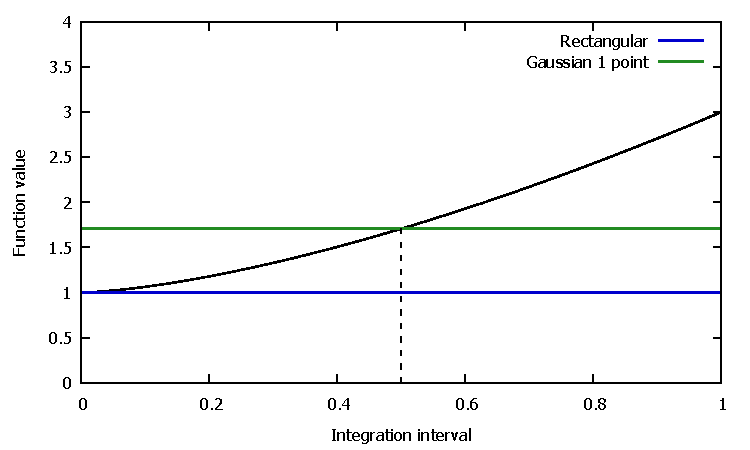
\includegraphics[width=6.53cm]{\FigDir/figure_gauss1.pdf}
  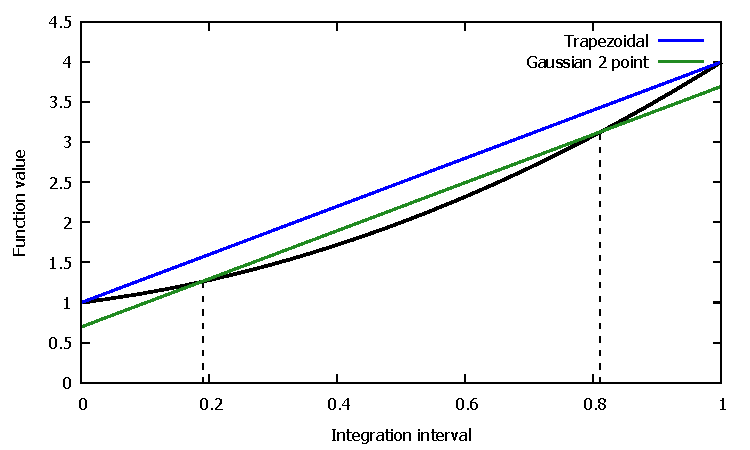
\includegraphics[width=6.53cm]{\FigDir/figure_gauss2.pdf}
  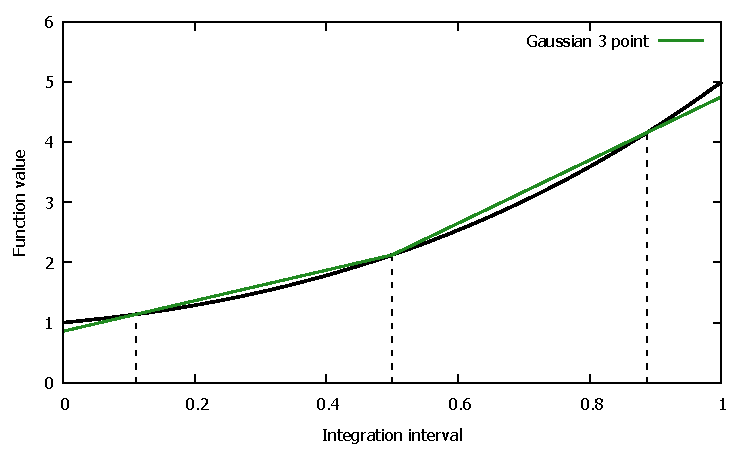
\includegraphics[width=6.53cm]{\FigDir/figure_gauss3.pdf}
\caption{Numerical integration methods for general use and the corresponding Gaussian
    methods for use when there is no feedback. 1 - Rectangular - Gaussian one point; 
    2 - Trapezoidal - Gaussian two point; 3 - Gaussian three point}
\end{figure}
     
The three points of the Gaussian numerical integration are situated symmetrical around x =
0, in order to integrate the interval [-0.5,0.5]. Therefore, one of the three function
evaluation points will be at the center, x=0. The other two points will be located at either
side of the Y-axis at distance $\gamma$ (so x=-$\gamma$ and x=$\gamma$). Now the interval [-0.5 ,0.5] is divided
in three parts, around these three points. The lengths of these sub-intervals determine the
weights which must be imposed on the Y-values corresponding to these three x-values and
considered representative for their sub-interval. Because of the symmetry again, the weights
belonging to -$\gamma$ and $\gamma$ are equal. When these weights are considered 1, the weight of the
central sub-interval is equal to $\omega$.

The values of the relative distance $\gamma$ and of the weight $\omega$ can be derived from the
requirement that both the second and the fourth order terms of the polynomial will be
exactly integrated (Goudriaan, 1986):

\begin{align*}
  & Numerical \ result  & Analytical \ result\\
  2^{nd} order \qquad&  
    \frac{(-\gamma)^{2} + 0 \cdot \omega  + \gamma^{2}}{1+\omega +1} &= 
    \int_{-\frac{1}{2}}^{-\frac{1}{2}} x^2 dx &= \frac{1}{12}   \\
  4^{th} order \qquad&  
    \frac{(-\gamma)^{4} + 0 \cdot \omega +\gamma^{4} }{1 +\omega +1} &=
    \int_{-\frac{1}{2}}^{-\frac{1}{2}} x^4 dx &= \frac{1}{80}   \\
\end{align*}



\begin{align*}
 2^{nd} order & & 4^{th} order\\
 \frac{(-\gamma)^{2} + \gamma^{2}}{1 + \omega + 1} &= {\frac{1}{12}} &
 \frac{(-\gamma)^{4} + \gamma^{4}}{1 + \omega + 1} &= \frac{1}{80} \nonumber  \\
 \frac{2 \gamma^{2}}{2 + \omega} &= \frac{1}{12} & 
 \frac{2 \gamma^{4}}{2 + \omega} &= \frac{1}{80} \nonumber \\
 24 \gamma^{2} &= 2 + \omega  & 160 \gamma^{4} &= 2n+ \omega
\end{align*}

Substitution yields the following values for the relative distance and the weight:

\begin{align*}
\gamma =\sqrt{{\frac{24}{160}}} = \sqrt{0.15}  \\
\omega = 1.6
\end{align*}

\section*{Examples of the use of Gaussian Integration in the model}

Canopy assimilation is calculated as a weighted average of the assimilation at three
horizons within the canopy. The leaf area index of the selected horizons can be calculated
as:

\begin{align*}
 L &=~(0.5~+~p \sqrt{0.15} )LAI \qquad where \ p~=~-1,0,1 \Rightarrow  \\
L_{1} &= 0.1127017 \cdot LAI  \\
L_{2} &= 0.5 \cdot LAI   \\
L_{3} &= 0.8872983 \cdot LAI
\end{align*}

The weighted average of the assimilation over the three selected horizons is: 

\begin{align*}
A_{h} = \frac{LAI(A_{-1} ~+~1.6A _{0} ~+~A _{1} )}{3.6} \Rightarrow   \nonumber  \\
A_{h} = LAI(0.2778A_{-1} ~+~0.4444A_{0} ~+~0.2778A_{1} )
\end{align*}

Where:\\[5pt]]
\begin{tabularx}{\textwidth}{llXr}   
A$_{{\rm h}}$ &:& Hourly canopy assimilation & [g CO$_{{\rm 2}}$ m$^{{\rm -2}}$ h$^{{\rm -1}}$]\\
\end{tabularx}

To integrate the instantaneous canopy assimilation over the day, again the Gaussian
approach of numerical integration is applied. The three selected points refer to the period
from noon to sun set. Daily canopy assimilation is obtained as the weighted average of the
instantaneous assimilation rates at the selected time points:

\begin{align*}
t_{h} &= 12 ~+~ 0.5D(0.5~+~p \sqrt{0.15} ) \qquad where \ p =-1,0,1 \\
A_{d} &= \frac{D(A_{h,-1} + 1.6A_{h,o} + A_{h,1})}{3.6}
\end{align*}

Where:\\[5pt]
\begin{tabularx}{\textwidth}{lcXr}
D &:& Day length     &    [h]\\
th &:& Hour of day   &     [h]\\
A$_{{\rm d}}$ &:& Daily canopy assimilation    & 
    [g CO$_{{\rm 2}}$ m$^{{\rm -2}}$ d$^{{\rm -1}}$]\\
\end{tabularx}